
\documentclass[10pt,twoside,slovak,a4paper]{article}

\usepackage{graphicx}
\graphicspath{ {./images/} }

\usepackage[slovak]{babel}
\usepackage[utf8]{inputenc}
\usepackage[IL2]{fontenc} 

\usepackage{graphicx}

\usepackage{url} 

\usepackage{hyperref}
\hypersetup{
    colorlinks=true,
    linkcolor=blue,
    filecolor=magenta,      
    urlcolor=blue,
    pdfpagemode=FullScreen,
}

\usepackage{wrapfig}

\usepackage{cite}

\usepackage{indentfirst}
\setlength{\parindent}{0.5cm}
% \usepackage{times}

\pagestyle{headings}



\date{\small 4. November 2022}

\begin{document}


\begin{titlepage}
	\title{Hra, ako nástroj pre edukáciu?
	\thanks{Semestrálny projekt v predmete Metódy inžinierskej práce, ak. rok 2022/23, vedenie: Ing. Igor Stupavský}} 
	\author{Svätopluk Puterka\\[2pt]
		{\small Slovenská technická univerzita v Bratislave}\\
		{\small Fakulta informatiky a informačných technológií}\\
		{\small \texttt{xputerkas@stuba.sk}}
	}
\end{titlepage}

{\maketitle }

\section{Úvod}
\begin{table}[!ht]
  \caption{Distribúcia videohráčov v USA v roku 2022}
   \centering
   \begin{tabular}{|l|l|}
   \hline
       Počet rokov & Podiel respondentov [\%] \\ \hline
       pod 18 rokov & 24 \\ \hline
       19-34 rokov & 36 \\ \hline
       35-44 rokov & 13 \\ \hline
       45-54 rokov & 12 \\ \hline
       55-64 rokv & 9 \\ \hline
       65+ rokov & 6 \\ \hline
   \end{tabular}
\end{table}
Počítačove hry sú v súčasnosti jedným z najväčších trhov na svete. Počet hodín strávených 
za hernými titulmi neustále rastie a taktiež rastie aj počet nových užívateľov hrajúcich 
herné tituly. Za posledné 3 roky sa situácia zmenila aj v školstve vplyvom pandémie COVID-19. Školy
boli zavraté a prezenčnú výučbu nahradilo distančné vzdelávanie. Učilia boli nútení k motivácii študentov využiť 
inovatívne riešenia k čomu výrazne pomohla gemifikácia výčbového procesu ~\cite{gemifikaciaPandemia, gemifikaciaNaSkole-1}.\\ 
Aj na základe vyššie spomenutých dát, ktoré budem neskoršie rozoberať v 
sekcii~\ref{data-o-hrani} by som sa chcel v tomto článku zamyslieť nad otázkou: 
„Je možne zvýšiť vzdelanie ludi hraním počítačových hier?“\\ 
V častiach~\ref{hry-na-skolach-hodiny-programovania} a~\ref{vytvorenie-vlastnej-hry} sa budem zaoberať 
tvorbou jednoduchých hier, ktorých cieľom bude naučenie sa nových spôsobov rozmýšľania nad problémami.
Záverečné poznámky opíšem v záverečnej časti~\ref{zaver}.
\section{Vytvorenie vlastnej hry}\label{vytvorenie-vlastnej-hry}

\begin{figure}
	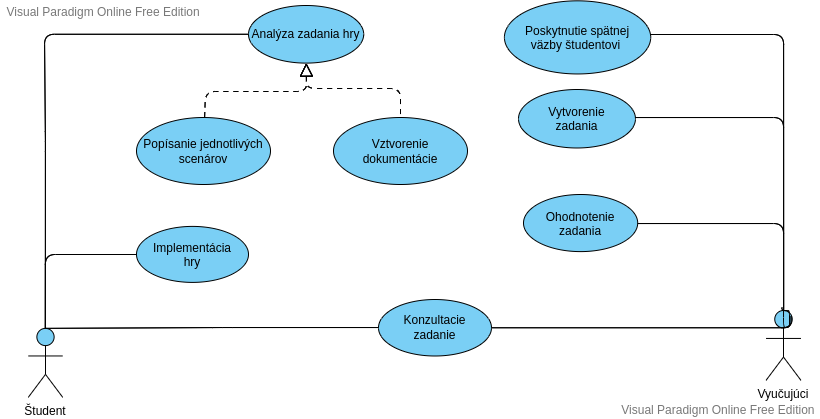
\includegraphics[width=\linewidth]{use-case.png}
	\caption{Use case diagram}
	\label{use-case-tvorba-hry}
\end{figure}


Okrem zakúpenia herných titulov, vytvorených pre vzdelávacie účely, si môžu študenti vytvárať aj vlastné hry.
Tento prístup má niekoľko výhod: 
	\begin{itemize}
		\item je aplikovateľný na širokú škálu ľudí a to s rôznymi úrovňami vedomostí
		\item ušetrenie finančných zdrojov, ktoré sú inak potrebné na kúpu herného titulu
		\item zlepšenie schopnosti spolupráce a rozdelenie jednotlivých úloh pri tímových úlohách 
	\end{itemize}

V tejto sekcii sa budem zameriavať hlavne na študentov stredných škôl.\\

Taktiež tvorba herného titulu bude vyžadovať kreativitu.
Zadania by si mohli študenti vymyslieť buď sami, alebo by si vybrali jednu z tém zadanú vyučujúcim.

Proces tvorby hry od návrhu až po vývoj pozostáva z rôznych úrovní, ktorými si musí jej tvorca prejsť.
Proces zadania hry by som rozdelil do dvoch hlavných častí:
	\begin{enumerate}
		\item \textbf{Analýza zadania a základných požiadaviek pre hru.}
		\item \textbf{Implementácia zadania.}
	\end{enumerate}

	% \subsection{Edukačné ciele zadania} 
	% Zadanie by malo byť tvorené

	\subsection{Analýza zadania a základných požiadaviek zadania.}\label{analyza-zadania}
	Cieľom analýzy základných požiadaviek zadania by malo byť porozumenie 
	daný požiadavkám a vyjasnenie si prípadných nejasností v zadaní. Analýza požiadaviek 
	hry sa môže skladať z na kreslenia základného diagramu požiadaviek,
	ktoré budeme musieť hra spĺňať pri práci v tíme. Pri analýze je taktiež potrebné komunikovať 
	s vyučujúcim o požiadavkách zadania. 


	\subsection{Implementácia zadania}\label{implementacia-zadania}
	\begin{enumerate}
		\item Analýza zadania hry
		\item Vytvorenie dokumentácie hry
		\item Popísanie jednotlivých scenárov
	\end{enumerate}


\section{Počítačove hry na školách}\label{hry-na-skolach-hodiny-programovania}
Idea vzdelávania detí prostredníctvom počítačových hier v školách by mohla naraziť na 
rôzne problémy v dnešnom vzdelávacom programe. Učitelia na školách majú málo času, sú striktne 
nastavené smernice a hodnotenie učiteľov je podmienené výkonom. Otázka by mohla nastať pri chýbajúcich 
vývojároch hier, ktorí by museli pravidelne konzultovať prípadné konfigurácie náročnosti úrovní, na 
základe menej porozumených oblastiach učiva. Musela by sa vyriešiť rôznorodá gramotnosť detí v informačných 
technológií, ktorý by mal určite rôzne úrovne, už len vzhľadom na rôznu finančnú situáciu rodín.\\\\\\
\indent~Vo všeobecnosti je náročné udržiavať pozornosť detí, ale aktívnym hraním by to bolo jednoduchšie~\cite{6624228}. Hry 
deťom spôsobujú radosť, čo by zvyšovalo motiváciu k učeniu. Ďalší aspekt, ktorý by priniesla táto metóda vzdelávania 
je rozvinutie kreativity pri riešení rôznych hádaniek. Okrem hier individuálneho charakteru zamerania sa 
by mohol byť istý druh počítačových hier orientovaný na riešenie problémov v skupinách, čo by podnecovalo 
lepšiu kooperáciu.\cite{7795662} Tieto získané schopnosti by boli prospešné v ich kariérnej budúcnosti.\\
\indent~Ako príklad by som uviedol školu \textbf{\href{https://www.q2l.org/}{Q2L-Quest to Learn}} v New York City, kde už v roku 2009 sa 
zrodila myšlienka učenie hrou a odvtedy na danej škole prebieha špeciálna výuka od 6. do 12. ročníka. 
Vyučovací proces prostredníctvom rôznych hier sa ukazuje, ako účinná alternatíva klasického vyučovania.
Pozorovanie na danej škole ukazuje, že u ich študentov zaznamenali väčšiu mieru kooperácie. Ako výhodu v úlohách uvádzajú 
možnosť opravy, ak žiaci v hre zlyhajú, a tým sa zvyšuje motivácia skúšať znova prejsť danú výzvu, naučiť 
sa a byť nakoniec úspešný. \\
V knihe ``Moderní vyučování`` od spisovateľa Geoffrey Petty ~\cite{pettyEd}, sa tiež hovorí, že podľa názoru humanistických psychológov je učenie 
najľahšie, zmysluplné a najúčinnejšie vtedy, keď prebieha v atmosfére zbavenej akejkoľvek hrozby. Žiaci by nemali byť motivovaní strachom 
z neúspechu, ale túžbou uspieť, dozvedieť sa viac.“ Pedagógovia si pochvaľujú rýchlu spätnú väzbu od žiakov na prebranú látku. 
V roku 2015 v ELA skúškach mali ich žiaci nadpriemerné výsledky medzi študentmi z rôznych škôl v rámci mesta.\\
\indent~Vďaka myšlienke zavedenia hier do školského vzdelávacieho systému by pri dostatočných predpokladoch mohli nastať pozitívne 
zmeny vo výsledkoch študentov, v čom sa ukazuje nový potenciál aplikácie gemifikácie na školy.



\section{Dáta o hraní hier}\label{data-o-hrani}
\section{Slabé a silné stránky učenia sa počítačovými hrami}\label{vyhody-nevyhody-hier}
\section{Záver} \label{zaver}

\bibliographystyle{plain} 
\bibliography{literatura}
\end{document}

